\chapter{Background}

Diabetes means that a patient must manually control their glucose levels. Glucose levels outside of normal levels, typically considered 4.0 mmol/L to 8.0 mmol/L pose a significant danger. Being below optimal -  \textbf{hypoglycaemia} - can cause unconsciousness and lasting brain damage within minutes. Being above optimal - \textbf{hyperglycaemia} -  can cause fatigue, thirst, headaches, etc in the short term. In the long term, it is very problematic and can lead to nerve damage and many chronic health issues such as nerve damage, blindness, and heart disease. 

\section{History}

While it has other applications, glucose measurement technology has always been driven by diabetes treatment and care. Diabetics need glucose measurements in order to inform immediate management, to analyze historical trends for future changes in care, and as a performance metric to measure whether they’ve met their goals. For the performance metric, glycated haemoglobin (HbA1c) measurements are most commonly used. This provides a rough average of glucose over the past three months. Everyday management, however, requires a user-friendly system that provides a good idea of the current location and behaviour of blood glucose.

Accurate glucose measurement is a key aspect of diabetes control, and has been developed for that purpose over the past century or so. Initially, it was measured through urine. This was a very crude method with poor accuracy and a significant time lag, so capillary blood glucose measurement took over in the form of fingerprick tests. While significantly more timely and accurate, these are uncomfortable and only provide a snapshot view. Subcutaneous Continuous Glucose Monitors, or CGMs, have been developed over the past decade to provide a semi-continuous (typically every 15 minutes) reading of interstitial fluid glucose levels. More systems have been sporadically developed, such as GlucoWatch, near infrared spectroscopy, and microdialysis. However, these have all fizzled out, usually because of issues with inaccuracy or user discomfort. Venous blood plasma is still in use, but due to the obvious impracticalities this is typically limited to hospital inpatients. This leaves capillary blood glucose spot checks and semi-continuous interstitial fluid monitoring as the current existing technology.  

Capillary blood glucose is considered the clinical gold standard. It’s easy to self-administer and quick to display changes in glucose level, making it the most responsive and up-to-date for patient management. Mostly, however, it has simply long been the only option. That means decades of medical practices have been developed using it for reference, so modern clinical care and diabetes management respond to venous blood information. It’s been institutionalized in. 

\begin{figure}[ht]
\centering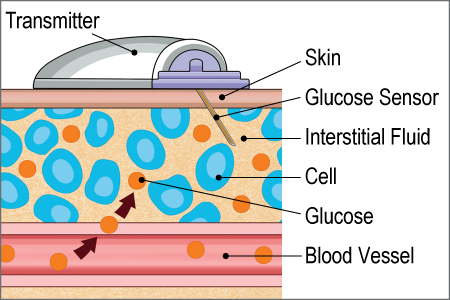
\includegraphics[width=0.5\linewidth]{images/cgm.png}
\caption{Illustration of a CGM sensor.}
\label{fig:cgmsensor}
\end{figure}

State-of-the-art ground truth measurement for glucose levels is typically ascribed to the Yellow Springs Instrument Glucose Analyzer, which measures venous plasma, but day to day use is handled through handheld Blood Glucose Meters (BGMs). Although accepted as ground truth in many studies, these are far from perfect. The accepted Diabetes Technology Society standard is that a BGM must be accurate to within 15\% at least 95\% of the time, and within 20\% at least 99\% of the time, compared to YSI readings \cite{noauthor_fda_2016}. Many meters do not meet this standard\footnote{A formal study on accuracy is \cite{clarke_evaluating_1987}, more recent informal studies are \cite{scheiner_2016_nodate},\cite{noauthor_are_2017},\cite{edelman_blood_2013}.}. Another popular assessment for BGMs is Clarke Error Grid Analysis (EGA). This is intended to measure clinical accuracy, or the likelihood that a glucose reading will provoke a detrimental management decision, and is equally important.

Over the past half decade, CGMs have been working their way into common practice. For immediate management, they give both an instantaneous spot check and an idea of current glucose behaviour, which is very helpful for tailoring action. On top of this, they also give semi-continuous historical data that can be used to get a better idea of glucose response to various environmental variables, which helps significantly in perfecting management. Analysis of this historical record can also lead to a more high definition performance metric.

Although CGMs directly measure interstitial fluid, their accuracy is judged by how close they are to blood glucose readings - officially to YSI, but most studies use BGM readings as an acceptable ground truth. A CGM accuracy will typically be reported as how close the spot checks are to a corresponding BGM reading. Although CGMs also give trend data, performance metrics for this are still being developed within the community. When it comes to clinical accuracy, the basic EGA is often used. However, Continuous Glucose Error Grid Analysis (CG-EGA) is in the late stage of development to judge the clinical accuracy of CGMs based on the wider range of information they provide. 

BGM capillary blood glucose is the accepted treatment basis for glucose management, because it’s the most reactive metric and already embedded in diabetes care. All other systems, regardless of how they sample glucose, strive to match it. However, continuous monitoring also provides a wealth of other useful information relevant to both diabetics and others.

\section{Sensor Choice}

Among the many commercially available sensors, we used Abbott’s Freestyle Libre. Among other reasons, it was the only one we could use. DexCom is not available in Singapore, and Medtronic only displays to an insulin pump. Being based in Singapore without an insulin pump, Abbott was the only option. It is not strictly speaking a CGM, since it doesn’t broadcast the results, which must be manually checked. Since that’s the only difference, for ease of reference it’s typically included under the umbrella term anyway.

\begin{figure}[ht]
\centering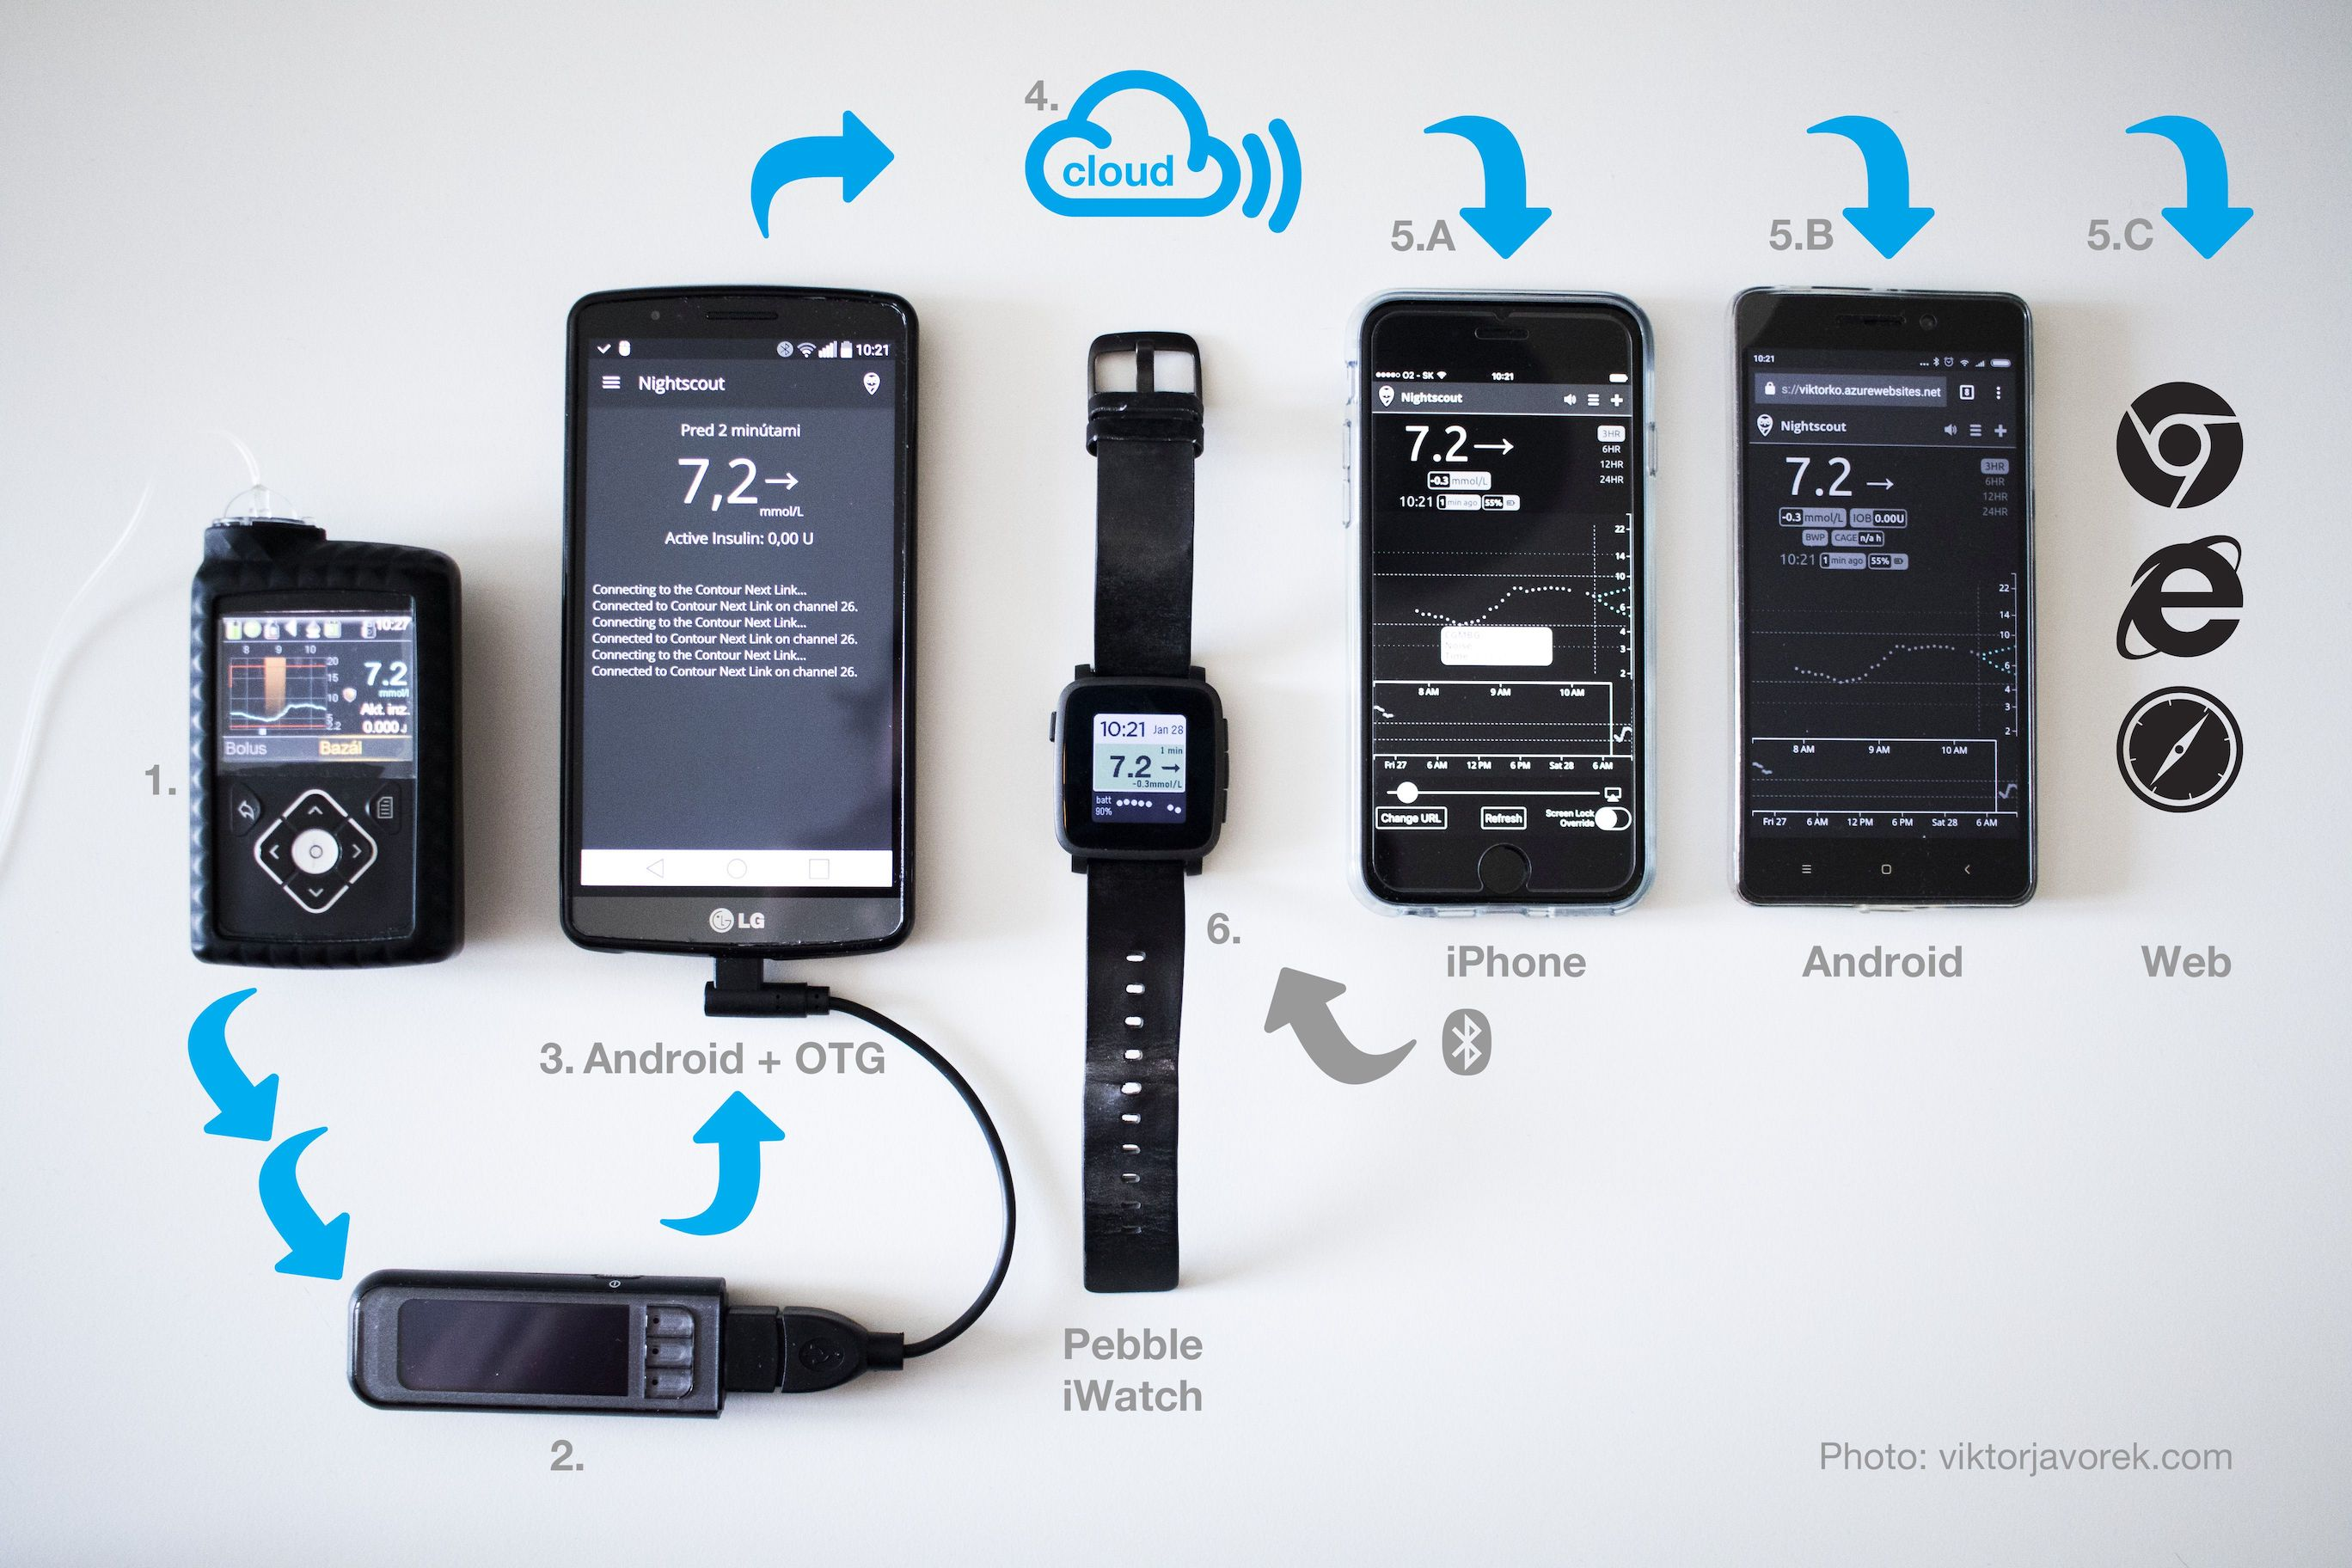
\includegraphics[width=1.0\linewidth]{images/nightscout}
\caption{The Nightscout ecosystem.}
\label{fig:nightscout}
\end{figure}

The Freestyle Libre has several other advantages. It is the cheapest and longest lived sensor available, with appreciable accuracy in all papers. The website is easily the most user-friendly, which is far more beneficial than it sounds. Most relevant to our purposes, it has the largest hacker community already formed. In particular, protocols and proof-of-concept software had been developed for accessing values straight from the sensor, and as we later found out, from the reader. Achieving something similar with DexCom apparently requires soldering together a xDrip device from scratch and online instructions. Data sent from sensor to display can be captured from both DexCom and Medtronic, with associated GitHub repositories. However, it’s more complicated and not intended for personal data analysis, being part of the bigger Nightscout\cite{noauthor_nightscout_nodate} project, which aims to provide a complete framework for managing glucose information.

\section{Freestyle Libre}
The Freestyle Libre CGM\footnote{It must be noted that the FreeStyle Libre is officially classified as a Flash Glucose Monitor (FGM), in that it does not alert the user directly, requiring a scan to do so. However, for the purposes of this report and the framework being built, we will use the terms CGM and FGM interchangeably.} consists of a subcutaneously implanted sensor and hand-held reader. Interstitial fluid readings are taken every 60 seconds, by the method described in detail below. The sensor records these raw values. Scanning the sensor with the reader automatically transmits the stored data through NFC. The reader then processes the raw data and displays a current glucose value, 8hr historical trend line, and an arrow indicating trend direction.

Studies have shown \cite{abbott_real-world_nodate} that using continuous glucose monitors (the Freestyle Libre in particular) have resulted in a 16\%reduction in HbA1c levels, as well as significantly lower occurrence and duration of hypoglycemic episodes. This is an extraordinarily positive result that lowers both short and long term risks due to diabetes complications by a significant margin.